%\documentclass[12pt]{article}
\documentclass[a0,landscape]{a0poster}

\usepackage{multicol} % This is so we can have multiple columns of text side-by-side
\columnsep=100pt % This is the amount of white space between the columns in the poster
\columnseprule=3pt % This is the thickness of the black line between the columns in the poster

\usepackage[font=small,labelfont=bf]{caption}

\usepackage{url}

\usepackage{amsmath}
\usepackage[dvips]{graphicx}
\usepackage{natbib}

\begin{document}

\begin{minipage}[b]{0.55\linewidth}
\veryHuge \textbf{Solving for multi-class}  % Title
\Huge\textit{A survey and synthesis}\\[1cm] % Subtitle
\huge \textbf{Peter Mills}\\ % Author(s)
\end{minipage}
%
\begin{minipage}[b]{0.25\linewidth}
	{\large 
	%\begin{tabular}{ll}
		Webpage:	\url{https://peteysoft.github.io}\\
		Software:	\url{https://github.com/peteysoft/libmsci}\\
		Email:		\textit{peteymills@hotmail.com}\\ % Email address
	%\end{tabular}
	}
\end{minipage}

\vspace{1cm}

\begin{multicols}{4}

\begin{abstract}
	\input{multiclass_review_abstract.txt}
\end{abstract}

Full paper:	\url{https://arxiv.org/abs/1809.05929}

\section*{Outline of the problem}

Many of the best statistical classifiers are {\it binary classifiers}, that is
they can only distinguish between two different classes, e.g.:
\begin{itemize}
	\item linear perceptrons
	\item logistic regression \citep{Michie_etal1994}
	\item support vector machines (SVM) \citep{Mueller_etal2001}
	\item piecewise linear classiifers \citep{Mills2018}
\end{itemize}

	{\bf Two problems:}

	\begin{enumerate}
		\item How do we partition the class labels so as to train the binary classifiers?

\item Given the estimated conditional probabilities of the binary classifiers:
	\begin{equation*}
		\lbrace P_i(c | \vec x) \rbrace
	\end{equation*}
want to find the conditional probabilities of the multi-class problem:
	\begin{equation*}
		P(j | \vec x), ~ j=[1..n_c]
	\end{equation*}
	\end{enumerate}

	{\bf Why use probabilities?}

\begin{enumerate}
  \item Provide useful extra information: quantify the accuracy of an estimate.
  \item Relation between binary and multi-class probabilities is unique and derives rigorously from probability theory.
  \item Binary classifiers that return a continuous decision function can be recalibrated to an approximate probability.
\end{enumerate}

\section*{Error correcting codes}

Use a {\it coding matrix}, $A$, to relate binary class probabilities to multi-class probabilities: \citep{Dietterich_Bakiri1995}
\begin{equation*}
	r_i = \frac{\sum_j a_{ij} p_j}{\sum_j |a_{ij} p_j}
\end{equation*}

\begin{itemize}
  \item $r_i=	P_i(+1|\vec x) - P_i(-1|\vec x)$
  \item $p_j = P(j|\vec x)$
\end{itemize}

Rearrange to form linear system:
\begin{eqnarray*}
Q \vec p & = & \vec r \\
q_ij & = & \left (1 - |a_ij| \right ) r_i
\end{eqnarray*}

\begin{itemize}
  \item $Q$ reduces to $A$ if $A$ contains no zeros.
  \item $A$ is transposed relative to normal convention: more natural when dealing with probabilities.
  \item All these equations derive rigorously from probability theory.
\end{itemize}

Example coding matrix, one-vs.-one:
\begin{equation*}
A =
\begin{bmatrix}
-1 & 1 & 0 & 0 \\
-1 & 0 & 1 & 0 \\
-1 & 0 & 0 & 1 \\
0 & -1 & 1 & 0 \\
0 & -1 & 0 & 1 \\
0 & 0 & -1 & 1
\end{bmatrix}
\end{equation*}

\section*{Decision trees}

Hierarchically subdivide the classes \citep{Lee_Oh2003}, such as in this hypothetical surface-classification probelm:

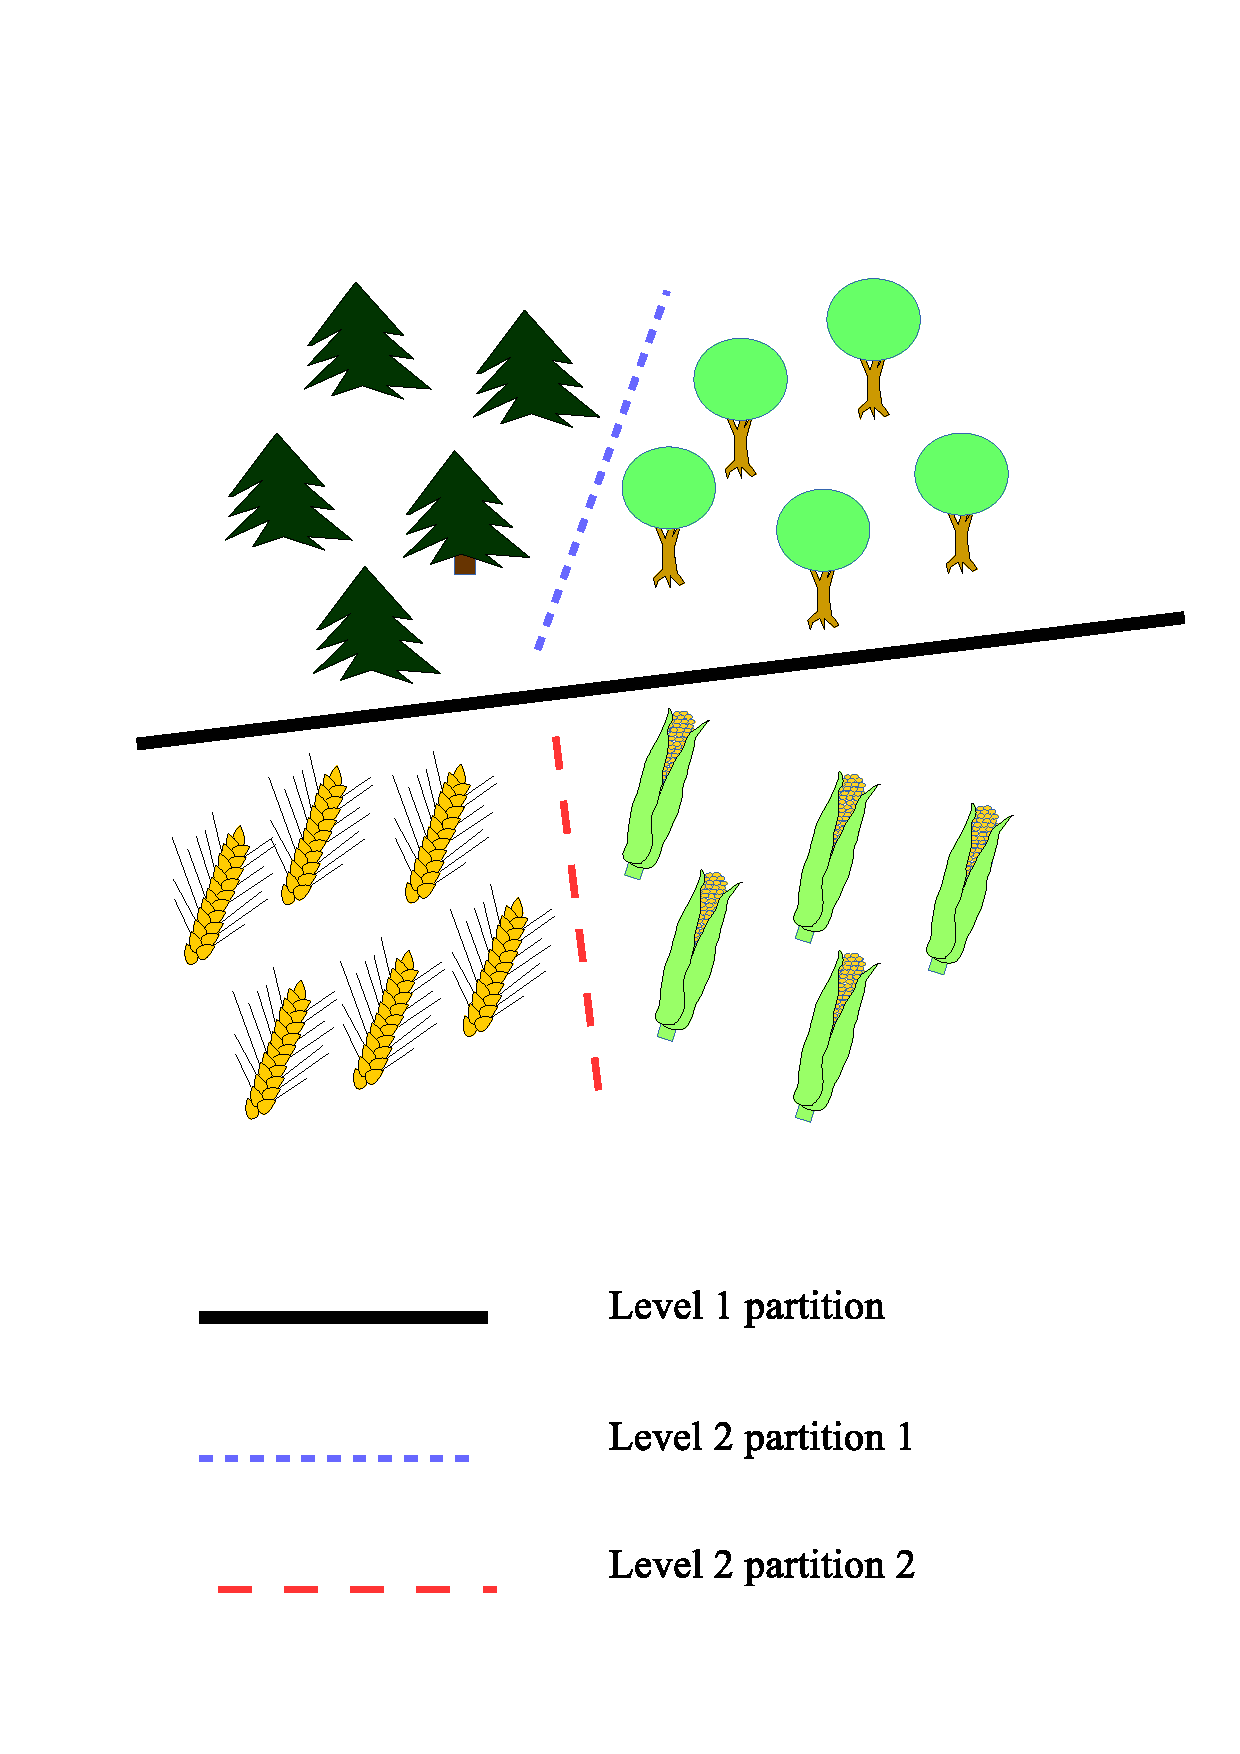
\includegraphics[width=0.15\textwidth]{landclasstree}

Only winning probability is returned as the
product of all the probabilities returned at each level.

\subsection*{Empirical decision trees}

\begin{itemize}
	\item Use inter-class distance to build dendrogram \citep{Benabdeslem_Bennani2006}.
	\item Hausdorff distance \citep{Ott1993}:
		\begin{equation*}
			D_{Hij} = \max \left \lbrace \min_k | \vec x_k - \vec x_l|~,~\min_l | \vec x_k - \vec x_l| ~ ;~y_k=i;~y_l=j \right \rbrace
		\end{equation*}
\end{itemize}

\section*{Unifying framework}

Recursive control language:

\begin{tabular}{lcl}
$<$branch$>$ & ::= & $<$model$>$ ``\{'' $<$branch-list$>$ ``\}'' $|$ $<$CLASS$>$\\
$<$model$>$  & ::= & $<$TWOCLASS$>$ $|$ $<$partition-list$>$\\
$<$branch-list$>$ & ::= & $<$branch$>$ $|$ $<$branch-list$>$ $<$branch$>$\\
$<$partition-list$>$ & ::= & $<$partition$>$ $|$ $<$partition-list$>$ $<$partition$>$\\
$<$partition$>$ & ::= & $<$TWOCLASS$>$ $<$class-list$>$ `` / '' $<$class-list$>$ ``;''\\
$<$class-list$>$ & ::= & $<$CLASS$>$ $|$ $<$class-list$>$ `` '' $<$CLASS$>$
\end{tabular}.

\begin{itemize}
\item $<$CLASS$>$ is a class value between $0$ and $n_c-1$.
\item $<TWOCLASS>$ is a binary classifier.
\end{itemize}

Example, one-vs.-one:

\begin{verbatim}
  model01 0 / 1;
  model02 0 / 2;
  model03 0 / 3;
  model12 1 / 2;
  model13 1 / 3;
  model23 2 / 3;
  {0 1 2 3}
\end{verbatim}

Example, the figure above:

\begin{verbatim}
  TreeVsField {
    EvergreenVsDeciduous {0 1}
    CornVsWheat {2 3}
  }
\end{verbatim}

The two methods, error-correcting-codes and decision trees, can be combined.
This is actually used in \citet{Zhou_etal2019}.

\section*{Numerical trials}

Six configurations:
\begin{itemize}
	\item 1-vs.-the-rest
	\item 1-vs.-1
	\item Orthogonal coding matrix \citep{Mills2017}
	\item ``Adjacent'' partitioning$^*$
	\item Arbitrary tree
	\item Empirically-designed tree
\end{itemize}

* Adjacent partitioning for seven classes:
\begin{verbatim}
  shuttle_adj-00 0 / 1 2 3 4 5 6;
  shuttle_adj-00 0 1 / 2 3 4 5 6;
  shuttle_adj-00 0 1 2 / 3 4 5 6;
  shuttle_adj-00 0 1 2 3 / 4 5 6;
  shuttle_adj-00 0 1 2 3 4 / 5 6;
  shuttle_adj-00 0 1 2 3 4 5 / 6;
  {0 1 2 3 4 5 6}
\end{verbatim}

Example of empirically-designed tree
for {\bf sat} dataset:
\begin{verbatim}
sat_emp {
  sat_emp.00 {
    sat_emp.00.00 {
      sat_emp.00.00.00 {
        sat_emp.00.00.00.00 {
          VERY DAMP GREY SOIL
          DAMP GREY SOIL
        }
        RED SOIL
      }
      GREY SOIL
    }
    STUBBLE
  }
  COTTON CROP
}
\end{verbatim}

\section*{Results}

Uncertainty coefficient \citep{Mills2018}:

{\small
%{\footnotesize
\begin{tabular}{|ll|llll|}
\hline
config. & method & letter & pendigits & usps & segment \\
\hline\hline
        1 vs. 1 & inv. & $\mathbf{0.940 \pm 0.002}$ & $\mathbf{0.986 \pm 0.003}$ & $\mathbf{0.931 \pm 0.009}$ & $0.922 \pm 0.010 $ \\
1 vs. rest & lsq. & $0.932 \pm 0.003 $ & $0.982 \pm 0.004 $ & $0.928 \pm 0.007 $ & $0.921 \pm 0.010 $ \\
        ortho. & iter. & $0.922 \pm 0.003^*$ & $0.982 \pm 0.003 $ & $0.927 \pm 0.008 $ & $\mathbf{0.923 \pm 0.010}$ \\
adj. & lsq. & $0.886 \pm 0.005 $ & $0.971 \pm 0.004 $ & $0.906 \pm 0.008 $ & $0.913 \pm 0.010 $ \\
hier & rec. & $0.880 \pm 0.004 $ & $0.972 \pm 0.004 $ & $0.910 \pm 0.007 $ & $0.909 \pm 0.008 $ \\
& lsq. & $0.888 \pm 0.004 $ & $0.973 \pm 0.004 $ & $0.912 \pm 0.007 $ & $0.909 \pm 0.008 $ \\
emp. & rec. & $0.905 \pm 0.003 $ & $0.979 \pm 0.003 $ & $0.917 \pm 0.008 $ & $0.903 \pm 0.006 $ \\
& lsq. & $0.910 \pm 0.003 $ & $0.979 \pm 0.004 $ & $0.920 \pm 0.010 $ & $0.909 \pm 0.007 $ \\
\hline
\end{tabular}
        \vspace{1 ex}

        $^*$ A random coding matrix was used since building an orthogonal matrix would take too long using current methods.

\begin{tabular}{|ll|llll|}
\hline
config. & method & sat & urban & shuttle & humidity\\
\hline\hline
        1 vs. 1 & inv. & $\mathbf{0.800 \pm 0.010}$ & $0.729 \pm 0.030 $ & $\mathbf{0.982 \pm 0.003}$ & $0.432 \pm 0.006 $ \\
1 vs. rest & lsq. & $0.799 \pm 0.009 $ & $0.728 \pm 0.030 $ & $0.979 \pm 0.003 $ & $0.359 \pm 0.007 $ \\
ortho. & iter. & $0.798 \pm 0.010 $ & $0.730 \pm 0.030 $ & $0.974 \pm 0.002 $ & $0.403 \pm 0.009 $ \\
        adj. & lsq. & $0.792 \pm 0.010 $ & $\mathbf{0.735 \pm 0.030}$ & $0.970 \pm 0.002 $ & $\mathbf{0.448 \pm 0.006}$ \\
hier & rec. & $0.788 \pm 0.010 $ & $0.724 \pm 0.030 $ & $0.974 \pm 0.003 $ & $0.435 \pm 0.006 $ \\
& lsq. & $0.789 \pm 0.010 $ & $0.727 \pm 0.030 $ & $0.973 \pm 0.002 $ & $0.433 \pm 0.007 $ \\
emp. & rec. & $0.790 \pm 0.009 $ & $0.702 \pm 0.050 $ & $0.977 \pm 0.004 $ & $0.440 \pm 0.008 $ \\
& lsq. & $0.795 \pm 0.010 $ & $0.714 \pm 0.040 $ & $0.975 \pm 0.003 $ & $0.437 \pm 0.008 $ \\
\hline
\end{tabular}
} % end \small

Brier score \citep{Jolliffe_Stephenson2003}:

{\small
\begin{tabular}{|l|llll|}
\hline
config. & letter & pendigits & usps & segment \\
\hline\hline
        1 vs. 1 & $\mathbf{0.0480 \pm 0.0008}$ & $\mathbf{0.032 \pm 0.002}$ & $\mathbf{0.066 \pm 0.003}$ & $0.090 \pm 0.005 $ \\
1 vs. rest & $0.0519 \pm 0.0007 $ & $0.035 \pm 0.002 $ & $0.070 \pm 0.003 $ & $0.092 \pm 0.004 $ \\
        ortho. & $0.0587 \pm 0.0006^*$ & $0.037 \pm 0.002 $ & $0.070 \pm 0.003 $ & $\mathbf{0.090 \pm 0.006}$ \\
adj. & $0.063 \pm 0.001 $ & $0.042 \pm 0.002 $ & $0.077 \pm 0.003 $ & $0.093 \pm 0.007 $ \\
hier. & $0.062 \pm 0.001 $ & $0.040 \pm 0.002 $ & $0.075 \pm 0.003 $ & $0.095 \pm 0.005 $ \\
emp. & $0.0553 \pm 0.0008 $ & $0.035 \pm 0.003 $ & $0.071 \pm 0.004 $ & $0.094 \pm 0.003 $ \\
\hline
\end{tabular}

\begin{tabular}{|l|llll|}
\hline
config. & sat & urban & shuttle & humidity\\
\hline\hline
        1 vs. 1 & $\mathbf{0.145 \pm 0.004}$ & $0.170 \pm 0.006 $ & $0.018 \pm 0.001 $ & $\mathbf{0.259 \pm 0.001}$ \\
        1 vs. rest & $0.149 \pm 0.003 $ & $0.171 \pm 0.007 $ & $\mathbf{0.012 \pm 0.001}$ & $0.2750 \pm 0.0009 $ \\
ortho. & $0.149 \pm 0.003 $ & $0.172 \pm 0.005 $ & $0.022 \pm 0.001 $ & $0.268 \pm 0.002 $ \\
        adj. & $0.152 \pm 0.004 $ & $\mathbf{0.167 \pm 0.008}$ & $0.0248 \pm 0.0007 $ & $0.264 \pm 0.002 $ \\
hier. & $0.150 \pm 0.004 $ & $0.167 \pm 0.007 $ & $0.023 \pm 0.001 $ & $0.259 \pm 0.001 $ \\
emp. & $0.149 \pm 0.004 $ & $0.173 \pm 0.008 $ & $0.022 \pm 0.001 $ & $0.261 \pm 0.002 $ \\
\hline
\end{tabular}
} %end \small

\section*{Conclusions}
\begin{itemize}
	\item One-size-fits-all method adequate for most datasets.
	\item One-vs.-one most accurate.
	\item Decision tree fastest (see full paper) \citep{Mills2018}.
	\item Some datasets benefit from a customized approach.
	\item Because the {\bf humidity} dataset is a discretized continuum problem there is an ordering to the classes, hence ``adjacent'' partitioning works best.
	\item Recursvie control language can help find best configuration.
\end{itemize}

\bibliographystyle{apa}

{\small
\bibliography{../agf_bib,multi2,../svm_accel/svm_accel,../pwl,../datasets}
}


\end{multicols}

\end{document}
